%!TEX root = ../dissertation.tex
\section{Representation of eye orientation in 3 dimensions}
\label{cha2:represent}
There are several ways of representing a rotation in 3D, the most common being euler angles and rotation matrices. Euler angles are three angles that describe the orientation of a rigid body with respect to a fixed coordinate system. However, in oculomotor research there are more suitable representations to use, such as quaternions or rotation vectors. \cite{rep}\cite{mathrot}

In computer vision, it's customary to use the coordinate system on the left of Figure \ref{cha2:sec2:fig:coordsys2}, but in neuroscience a different convention, represented on the right of the Figure, is used. In order to be coherent with computer vision concepts, the first mentioned convention will be the one in use throughout the remaining of this section.

\begin{figure}[!htb]
	\centering
		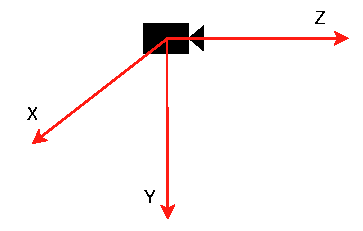
\includegraphics[width=0.41\textwidth]{images/cvcoordinatesys.pdf}
		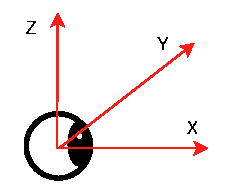
\includegraphics[width=0.25\textwidth]{images/cvcoordinatesysq.pdf}
		\caption[Computer Vision vs Neuroscience coordinate systems]{On the left, the coordinate system used in computer vision with the torsional component coming out of the front of the camera. On the right, the coordinate system used in the neuroscience field with the torsional component coming out of the front of the eye.}
		\label{cha2:sec2:fig:coordsys2}
\end{figure}

\subsection{Rotation matrices}
\label{rotmatsss}
The eye is a rotating body (no translations), and thus any orientation can be described by a unique series of three rotations around each of the axis defined in three dimensional space as
\begin{equation}
\label{rrr}
R _ { x } ( \psi ) = \left[ \begin{array} { c c c } { 1 } & { 0 } & { 0 } \\ { 0 } & { \cos \psi } & { - \sin \psi } \\ { 0 } & { \sin \psi } & { \cos \psi} \end{array} \right], \
R _ { y } ( \phi ) = \left[ \begin{array} { c c c } { \cos \phi } & { 0 } & { \sin \phi } \\ { 0 } & { 1 } & { 0 } \\ { - \sin \phi } & { 0 } & { \cos \phi } \end{array} \right], \
R _ { z } ( \theta ) = \left[ \begin{array} { c c c } { \cos \theta } & { - \sin \theta } & { 0 } \\ { \sin \theta } & { \cos \theta } & { 0 } \\ { 0 } & { 0 } & { 1 } \end{array} \right],
\end{equation}
where each angle is defined in counter-clockwise direction around each axis. An arbitrary rotation, $R$, may then be defined as some multiplication (i.e. a serial order) of those three, noting that the order by which they are multiplied matters (rotations are non-commutative). A matrix originated from any combination of those is a rotation matrix because it satisfies the following conditions,
\begin{align}
	R^{-1} = R^T\\
	det(R) = 1.
\end{align} 

Instead of using multiple rotations done  after each other, Euler's theorem states that the orientation of the rotating body can also be parametrized by a single rotation with an angle, $\rho$, about an axis in 3D, $\hat{\mathbf{n}} = (n_1, n_2, n_3)$. That rotation is denoted as $R(\hat{\mathbf{n}}, \rho)$ and is given by 
\begin{equation}
R ( \hat { \mathbf{n} } , \rho ) = \left( \begin{array} { c c c } { \cos \rho + n _ { 1 } ^ { 2 } ( 1 - \cos \rho ) } & { n _ { 1 } n _ { 2 } ( 1 - \cos \rho ) - n _ { 3 } \sin \rho } & { n _ { 1 } n _ { 3 } ( 1 - \cos \rho ) + n _ { 2 } \sin \rho } \\ { n _ { 1 } n _ { 2 } ( 1 - \cos \rho ) + n _ { 3 } \sin \rho } & { \cos \rho + n _ { 2 } ^ { 2 } ( 1 - \cos \rho ) } & { n _ { 2 } n _ { 3 } ( 1 - \cos \rho ) + n _ { 2 } \sin \rho } \\ { n _ { 1 } n _ { 3 } ( 1 - \cos \rho ) - n _ { 2 } \sin \rho } & { n _ { 2 } n _ { 3 } ( 1 - \cos \rho ) + n _ { 1 } \sin \rho } & { \cos \rho + n _ { 3 } ^ { 2 } ( 1 - \cos \rho ) } \end{array} \right).
\end{equation}


\subsection{Rotation axis and angle}
There are multiple ways by which to obtain the axis and angle of the rotation matrix. The following one uses the fact that a vector, $\mathbf{r}$, parallel to the rotation axis, $\hat{\mathbf{n}}$, is necessarily an eigenvector of the rotation matrix with the eigenvalue $\lambda = 1$, as described by
\begin{equation}
\label{fu}
R \mathbf{r} = \mathbf{r}.
\end{equation}
Rewriting (\ref{fu}) as $( R - I ) \mathbf{r} = 0$, it can be shown that 
\begin{equation}
\label{fff}
0 = R ^ { T } 0 + 0 = R ^ { T } ( R - I ) \mathbf{r} + ( R - I ) \mathbf{r}  = \left( R ^ { T } R - R ^ { T } + R - I \right) \mathbf{r} = \left( I - R ^ { T } + R - I \right) \mathbf{r} = \left( R - R ^ { T } \right) \mathbf{r}.
\end{equation}
Because $(R - R^T)$ is a \gls{skews}, $\mathbf{r}$ may be chosen such that $[ \mathbf{r} ] _ { \times} = \left( R - R ^ { T } \right)$, and (\ref{fff}) then becomes a cross-product of vector $\mathbf{r}$ with itself,
\begin{equation}
\left( R - R ^ { \mathrm { T } } \right) \mathbf{r} = [ \mathbf{r} ] _ { \times } \mathbf{r} = \mathbf{r} \times \mathbf{r} = 0,
\end{equation}
obtaining
\begin{equation}
\label{gggggg}
\mathbf{r} = \left( \begin{array} { c } { R _ { 32 } - R _ { 23 } } \\ { R _ { 13 } - R _ { 31 } } \\ { R _ { 21 } - R _ { 12 } } \end{array} \right),
\end{equation}
as the rotation axis. This does not work if $R$ is symmetric, to do so, it is necessary to diagonalize the matrix and find the eigenvector which corresponds to the eigenvalue of 1.

The rotation angle can be obtained through $\| \mathbf{r} \| = 2 \sin \rho$, or through a more direct method by computing the trace of $R(\hat{\mathbf{n}}, \rho)$, defined as
\begin{equation}
\operatorname { Tr } R ( \hat { \mathbf{n} } , \rho ) = 1 + 2 \cos \rho.
\end{equation}


\subsection{Rotation vector in head-fixed coordinates}
\label{killme}
There are other ways to represent a rotation that may be more appropriate for this work, such as the next one, which comes from neuroscience. Here, there is a rotation vector, $\mathbf{r}$, directed along the rotation axis, $\hat{\mathbf{n}}$, which length varies with the amount of rotation, $\rho$, around it. A description of this vector is given by 
\begin{equation}
\mathbf{r} = \tan (\frac{\rho}{2}) \hat{ \mathbf{n}},
\end{equation}
that can be obtained through the previous rotation vector (\ref{gggggg}) as 
\begin{equation}
\label{sec2:eq:n}
\begin{aligned} 
\cos \rho & = 1 / 2 \cdot \left( R _ { 11 } + R _ { 22 } + R _ { 33 } - 1 \right) \\ 
n_ { x } & = \sin \rho \left( R _ { 32 } - R _ { 23 } \right) / 2  \\ 
n _ { y } & = \sin \rho \left( R _ { 13 } - R _ { 31 } \right) / 2  \\ 
n _ { z } & = \sin \rho \left( R _ { 21 } - R _ { 12 } \right) / 2  .
\end{aligned}
\end{equation}
It's important to note that in this format, the units are given in half-radians.

\subsection{Quaternions}
\label{cha2:represent:quat}
Quaternions are 4-dimensional complex algebraic objects that are related to a rotation around an axis, $\hat{ \mathbf{n}}$, just like the representation before, by an angle $\rho$ as follows,
\begin{equation}
\label{sec2:eq:q}
q = \cos ( \rho / 2 ) + i \sin ( \rho / 2 ) \hat{n} \equiv q _ { 0 } + {\bf i}\cdot  {\bf q},
\end{equation}
where $q_0$ and ${\bf q}$ are the scalar and vectorial parts of the quaternion, respectively, and ${\bf i}$ is the complex 3D vector. For the description of eye movements, only the vectorial part is necessary. Quaternions are related to rotation vectors by $ \mathbf{r}  = {\bf q} / q _ { 0 }$.
\cite{rep}

ADD MULTIPLICATION WITH ROTATION
